\chapter{Artifact Classification}\label{Ch:classification}


In order to classify the artifacts we considered a variety of machine learning algorithms, under both supervised and unsupervised categories. Supervised learning algorithms use labeled data to learn how to classify the data based on the given labels (categories), while unsupervised models infer patterns in the data without referring to the labels. Here we discuss the different algorithms that we tried in order to perform a binary classification (corrupted vs. normal) on our data.

\section{Classical Machine Learning Methods}\label{classic}
In order to train supervised algorithms, we need labeled data. In other words, for each training instance, we need to know whether it is corrupted and what type of artifact it contains. Since we have collected normal images and produced corrupted images, we are ready to train supervised learning algorithms:

\subsection{Linear Discriminant Analysis (LDA)}

In our study, we have used the two-class linear discriminant analysis (LDA) \cite{scikit-learn} as one of the individual artifact detection models. Consider the set of features $\Vec{x}$ for each sample and its associated label $y$. To predict class labels given a specific set of features $\Vec{x}$, we look at the log-likelihood ratio,
$$ \log\left( \frac{P(y=0 | \Vec{x})}{P(y=1 | \Vec{x})} \right) = \log\left( \frac{P(\Vec{x}| y = 0) P(y = 0)}{P(\Vec{x}| y = 1) P(y = 1)} \right)$$
LDA assumes that the conditional probability density functions $P(\Vec{x} | y = 0)$ and  $P(\Vec{x} | y = 1)$ are both normally distributed with mean and covariance $(\Vec{\mu_0}, \Sigma_0)$ and $(\Vec{\mu_1}, \Sigma_1)$, estimated from the training data. Also, we can estimate $P( y = 0)$ and $P( y = 1)$ by the proportion of samples from class $0$ or $1$. In the LDA case, we further assume that the Gaussian distributions for each class share the same covariance matrix, so $\Sigma_0 = \Sigma_1 = \Sigma$. Using the multivariate Gaussian assumption, we will predict class label 0 if:

\begin{equation*}
\begin{split}
    & \log\left( \frac{P(y=0 | \Vec{x})}{P(y=1 | \Vec{x})} \right)  > 0 \\
    \iff & \log\left( \frac{P(\Vec{x}| y = 0) P(y = 0)}{P(\Vec{x}| y = 1) P(y = 1)} \right) > 0 \\
    \iff & (\Vec{\mu_0} - \Vec{\mu_1})^t \Sigma ^{-1} \Vec{x} > \frac{1}{2} (\Vec{\mu_0}^{t} \Sigma^{-1} \Vec{\mu_0} - \Vec{\mu_1}^{t} \Sigma^{-1} \Vec{\mu_1} ) -\log \frac{P(y=0)}{P(y=1)}
\end{split}    
\end{equation*}



\subsection{Support Vector Machine (SVM)}

Consider the case where there are two classes of data (blue and green) that are linearly separable:

\begin{figure}[H]
    \centering
    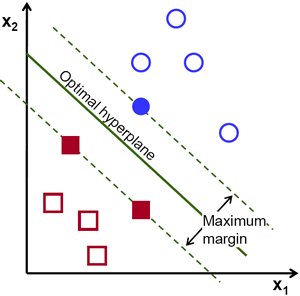
\includegraphics[scale=2.0]{images/svm.png}
  % \centering
    \caption{2-D Linearly Separable Data.}
    \label{ls-svm}
\end{figure}

\noindent Support vector machine compute the decision boundary that maximizes the margin, which is defined as the distance of the closest data point to the decision boundary \cite{Cortes95support-vectornetworks}. Mathematically, support vector machine is a function $f: \mathbb{R}^m \rightarrow \{1,-1\}$, where $m$ is the dimension of the data, and $1$ and $-1$ correspond to the two classes. Suppose the number of data is $n$, then the function $f$ is given by:
$$\Scale[1.2]{f(x) = \text{sign} (\mathbf{w}\mathbf{x}+\mathbf{b})}$$ where $\mathbf{w}$ and $\textbf{b}$ are solutions to the following optimization problem:
$$\Scale[1.2]{\begin{array}{ll}{\min _{\mathbf{w}, b}} & {\frac{1}{2} \mathbf{w}^{\top} \mathbf{w}} \\ {\text { s.t. }} & {y_{i}\left(\mathbf{w}^{\top} \mathbf{x}_{i}+b\right) \geq 1, \quad i=1, \ldots, n }\end{array}} $$

\noindent The optimization problem is typically solved via its dual problem. In the case where the data is not linearly separable, there is no solution to the optimization problem above. Therefore we add slack variables $\xi_i \; \forall i = 1,2, \ldots, n$ to the problem, which allows data points to be within the margin \cite{soft_svm}:
$$\Scale[1.2]{\begin{array}{c}{\min _{w, b, \xi \geq 0} \frac{1}{2} \mathbf{w}^{\top} \mathbf{w}+C \sum_{i} \xi_{i}} \\ {\text { s.t. } y_{i}\left(\mathbf{w}^{\top} \mathbf{x}_{i}+b\right) \geq 1-\xi_{i}, \quad i=1, \ldots, n}\end{array}}$$

\noindent The SVM algorithm can be generalized to classify more than two classes. There are also many other supervised learning algorithms such as random forest and convolutional neural network that can be applied to identify corrupted images. We expect them to perform well in identifying known artifacts. On the other hand, supervised algorithms will probably not able to detect unknown artifacts. As a result, we also consider applying unsupervised algorithms.


\subsection{Logistic Regression}
One of the most commonly used statistical tools for binary classification is logistic regression which is an extension to linear regression. As opposed to linear regression which fits a straight line or a hyperplane to the data, logistic regression uses the logistic function to squeeze the output of a linear equation between 0 and 1, thereby producing a probability \cite{logistic}. The logistic function is defined the following:

\begin{equation}
\operatorname{logistic}(\eta)=\frac{1}{1+\exp (-\eta)}
\label{logistic}
\end{equation}

\begin{figure}[H]
    \centering
    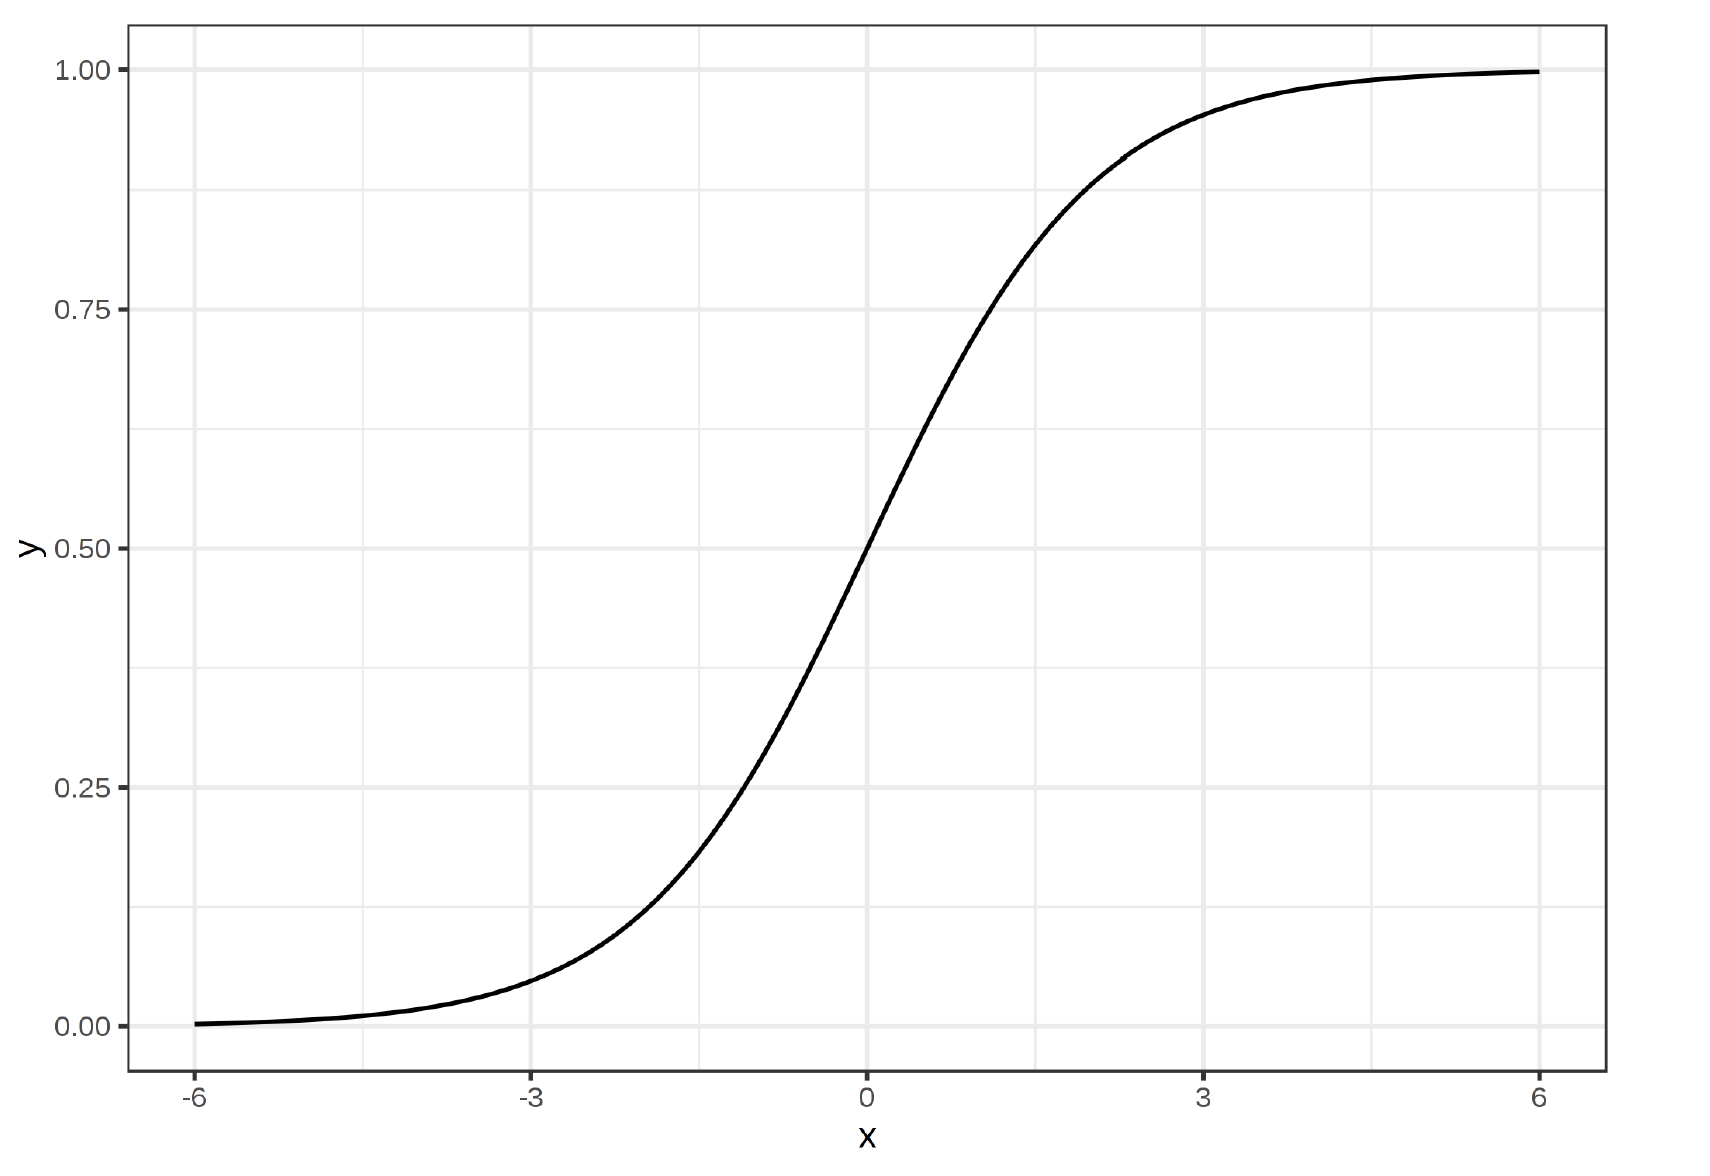
\includegraphics[scale=0.3]{images/log.png}
    \caption[Logistic Function]{Logistic (sigmoid) function maps the input to a number between 0 and 1.}
    \label{log}
\end{figure}

\noindent
Similar to linear regression where the model learns the weights $\beta_i$ that minimize the prediction error (illustrated in Equation \eqref{linear}), logistic regression minimizes the loss function, with the linear model given as input to the logistic function in order to produce a number between 0 and 1 (see Equation \eqref{log_eq}). Gradient decent is used to find the minimum of the loss function.


\begin{equation}
\hat{y}^{(i)}=\beta_{0}+\beta_{1} x_{1}^{(i)}+\ldots+\beta_{p} x_{p}^{(i)}
\label{linear}
\end{equation}

\begin{equation}
P\left(y^{(i)}=1\right)=\frac{1}{1+\exp \left(-\left(\beta_{0}+\beta_{1} x_{1}^{(i)}+\ldots+\beta_{p} x_{p}^{(i)}\right)\right)}
\label{log_eq}
\end{equation}


%%%%%%%%%%%%%%%%%%%%
\newpage
%%%%%%%%%%%%%%%%%%%%

\section{Deep Learning Methods}\label{deep}

\subsection{Convolutional Neural Network}

\noindent Convolutional Neural Network (CNN) is a class of deep neural networks which are often applied to analyzing visual imagery \cite{cnn_anomaly1}\cite{cnn_anomaly2}. Compared to other image classification algorithms, CNN requires relatively little pre-processing since it is able to automatically extract features from the training data.\\

\noindent A convolutional neural network consists of several types of layers, including fully connected layer, convolutional layer, and pooling layer \cite{cnn}. In a fully connected layer, each neuron is connected to every neuron in the previous layer. In a convolutional layer, however, each neuron is connected to a restricted subarea of the previous layer. Pixels within the subarea are convolved with a filter whose parameters are learned during the training step, and the result is passed to the corresponding neuron in the convolutional layer. Moreover, pooling layers reduce the dimensions of the data by combining the values in a subarea in the previous layer into a single neuron in the pooling layer. For instance, max pooling uses the maximum value within each subarea, and average pooling uses the average value within each subarea.\\

\begin{figure}[h]
\captionsetup{}
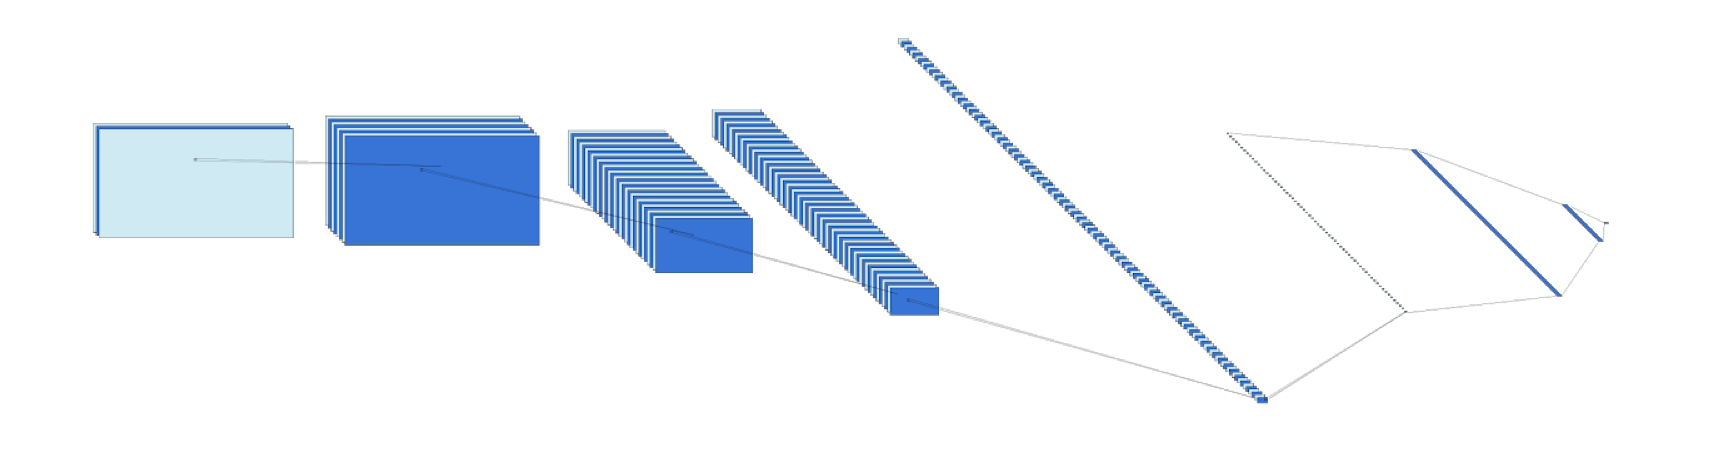
\includegraphics[scale=0.5]{images/cnn_structure.png}
\caption[Structure of our CNN model]{Structure of our CNN model. There are 5 convolutional layers, each followed by a max pooling layer. The two layers before the final output layers are fully connected.}
\label{fig:cnnstructure}
\end{figure}


\noindent Similar to other deep learning models, CNN is trained using back-propagation. We choose cross-entropy \cite{loss_function} as the loss function for our model, which is defined by:
$$ g(x) = - l_t (x) \log l_p (x) - (1-l_t (x)) \log (1 - l_p(x))$$

\noindent where $l_t(x) \in \{0,1\}$ is the true label of instance $x$ and $l_p(x) \in \{0,1\}$ is the predicted label of instance $x$ (here normal class corresponds to label 0, and corrupted class corresponds to label 1). The parameters of the model are updated through gradient descent in order to minimize the loss function. During testing, each instance is fed into the CNN, and the model outputs the probability that the instance is corrupted.\\

\subsection{Generative Adversarial Network}

\noindent Generative Adversarial Network has been a popular area of research in deep learning during recent years. We consider to apply GAN to detect artifacts because it only requires normal images as training data. GAN consists of two components: a generator $G$ and a discriminator $D$. The generator is supposed to take in random noise and generate fake images that resemble training data, and the discriminator is supposed to distinguish images produced by the generator from the training data \cite{gan}. \\


\begin{figure}[h]
\centering
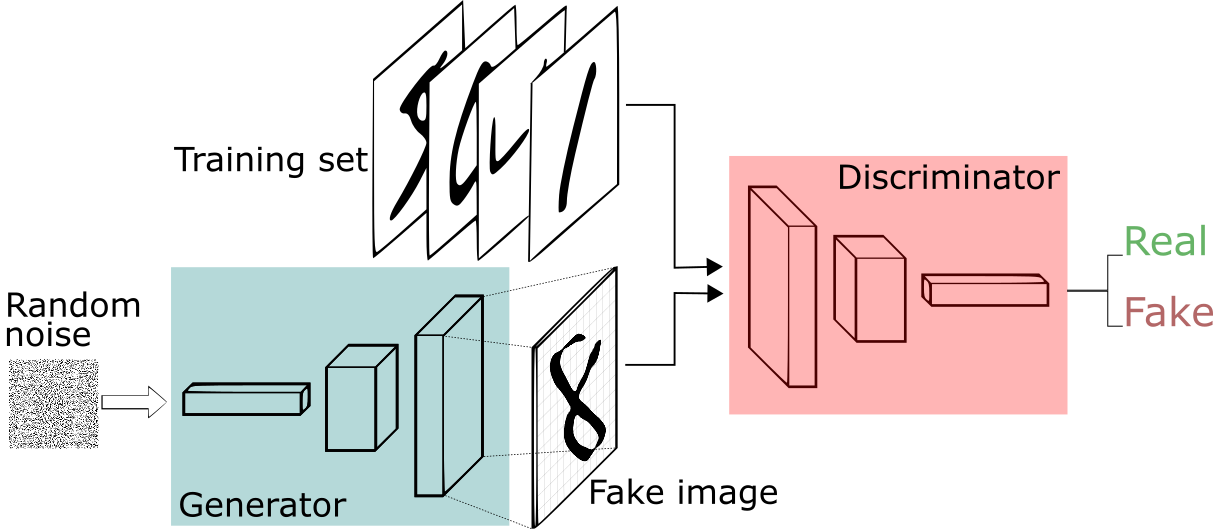
\includegraphics[scale=0.3]{images/gan.png}
\caption{Structure of a GAN.}
\label{fig:structureGAN}
\end{figure}

\noindent The model's loss function is defined by:

$$
\min _{G} \max _{D} V(D, G)=\mathbb{E}_{\boldsymbol{x} \sim p_{\text {data }}(\boldsymbol{x})}[\log D(\boldsymbol{x})]+\mathbb{E}_{\boldsymbol{z} \sim p_{\boldsymbol{z}}}(\boldsymbol{z})[\log (1-D(G(\boldsymbol{z})))]
$$

\noindent The two components in a GAN are trained an iterative numerical approach. When training the discriminator $D$, the parameters in the generator, $\theta^{(D)}$, are held fixed, and the parameters in $G$, $\theta^{(G)}$, are updated using gradient ascent to maximize the loss function:

$$\theta^{(D)} \leftarrow \underset{\theta^{(D)}}{\arg \max }\left[ \mathbb{E}_{x \sim p_{\text {data }}} \log D(\mathbf{x})+ \mathbb{E}_{\mathbf{z}} \log (1-D(G(\mathbf{z})))\right]$$

\noindent When training the generator, $\theta_D$ are held fixed, and $\theta_G$ are updated using gradient descent to minimize the loss function:

$$\theta^{(G)} \leftarrow \underset{\theta^{(G)}}{\arg \min }  \mathbb{E}_{\mathbf{z}} \log (1-D(G(\mathbf{z})))$$

\noindent It can be shown that a unique global optimal solution exists, where the generator learns the distribution of the training data and the discriminator outputs the probability of the input image being real as $\frac{1}{2}$ all the time, which indicates that it is not able to distinguish fake images produced by the generator from the training data.\\


\noindent Most research done on GAN focuses on the generator \cite{style_gan}. However, we think the discriminator may be able to identify anomalous images that are different from the training data. Therefore we use a generative adversarial model that are trained on normal data to detect artifacts.
%%%%%%%%%%%%%%%%%%%%
\newpage
%%%%%%%%%%%%%%%%%%
\section{Ensemble Methods}
Initially, we approached the classification stage by training a single CNN model that would discriminate between corrupted images (regardless of the artifact type) from normal. However, the unsatisfactory performance suggested that a single model might be unable to capture cross-class patterns in the scope of this project. Thus, we switched to a mixed experts ``ensemble'' model that combines multiple learning algorithms, each of which specializes in identifying one particular artifact type. Our classification procedures can thus be described as follows.

\begin{enumerate}
    \item \textbf{Training Stage 1.} First, we trained the individual models for binary classification for each corruption type. For this training procedure, we extracted images from 24 games (dataset $A$ in Table \ref{games}), kept 2,400 of those images as normal and applied \texttt{Glitchify} to the rest, obtaining around 1,500 frames per corruption type. A variety of models introduced in Sections \ref{classic} and \ref{deep} were paired with features from Chapter \ref{Ch:feature} and trained as binary classifiers for each artifact type from Chapter \ref{Ch:datagen}. The best models were then selected and their performances were recorded in Table \ref{tab:models}. Table \ref{fig:methods-tried} shows all pairings ``artifact-feature-model'' that were considered in the scope of this project.
    
    \item \textbf{Training Stage 2:} after putting together the individual trained models, we train a logistic regression on the output of the individual models concatenated together. At this stage, our dataset comprised of 3 games (dataset $B$ in Table \ref{games}) - never seen by the individual models - with 1650 normal images and 150 images of each type of artifact. A 0.25/0.75 test-train split was applied to the data. At this stage, all of the models are given normal images in addition to all types of artifacts. The performance on the test set is reported in Table \ref{tab:stage2}.
    \item \textbf{Testing:} the goal of this stage is to measure the generalizability of the ensemble model. That is, how well the ensemble performs on games it has never seen before. The heldout test set was composed of 3 games (see dataset C in Table \ref{games}), with 1650 normal images and 1800 corrupted images, which is 150 for each artifact type. All of these images were used to test the ensemble. The results are reported in Tables \ref{tab:variation} and \ref{tab:test_models}.
\end{enumerate}

\newpage

\begin{figure}[!h]
  \centering
  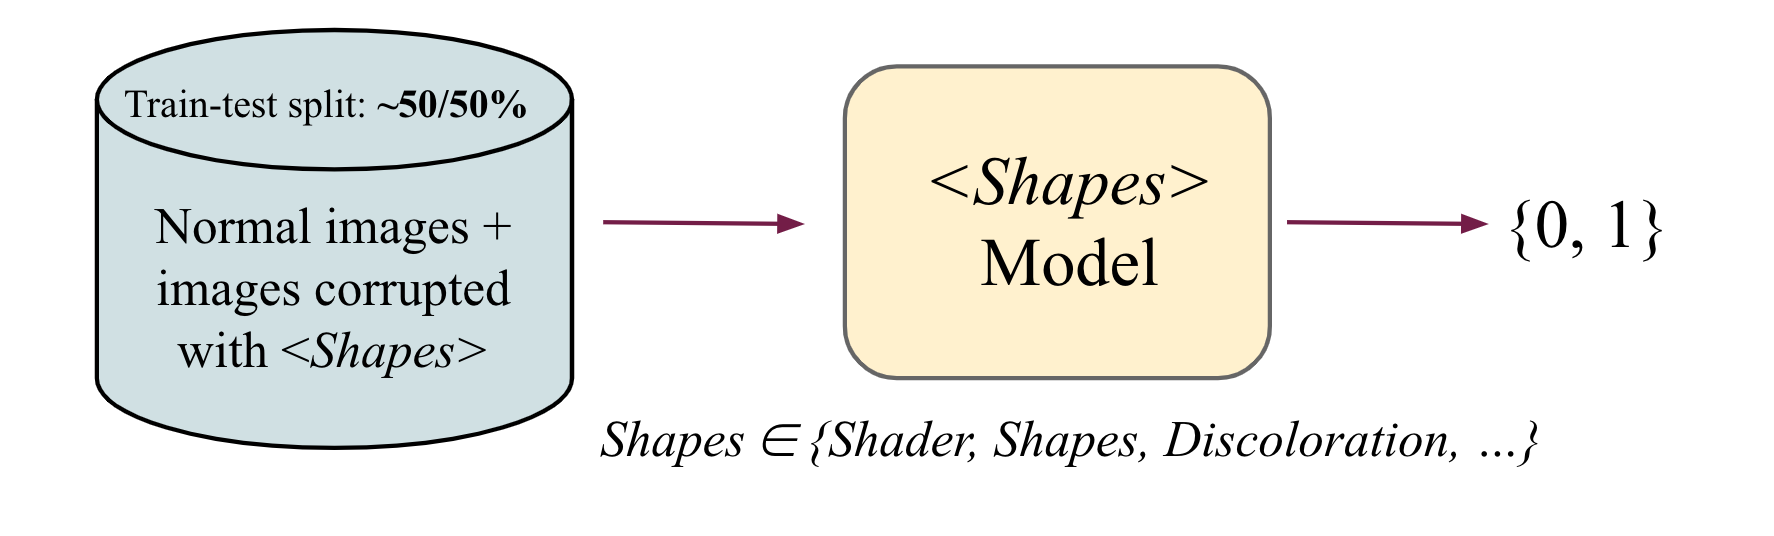
\includegraphics[scale=0.3]{images/stage_1.png}
  \caption*{Training Stage 1.}
  \centering
  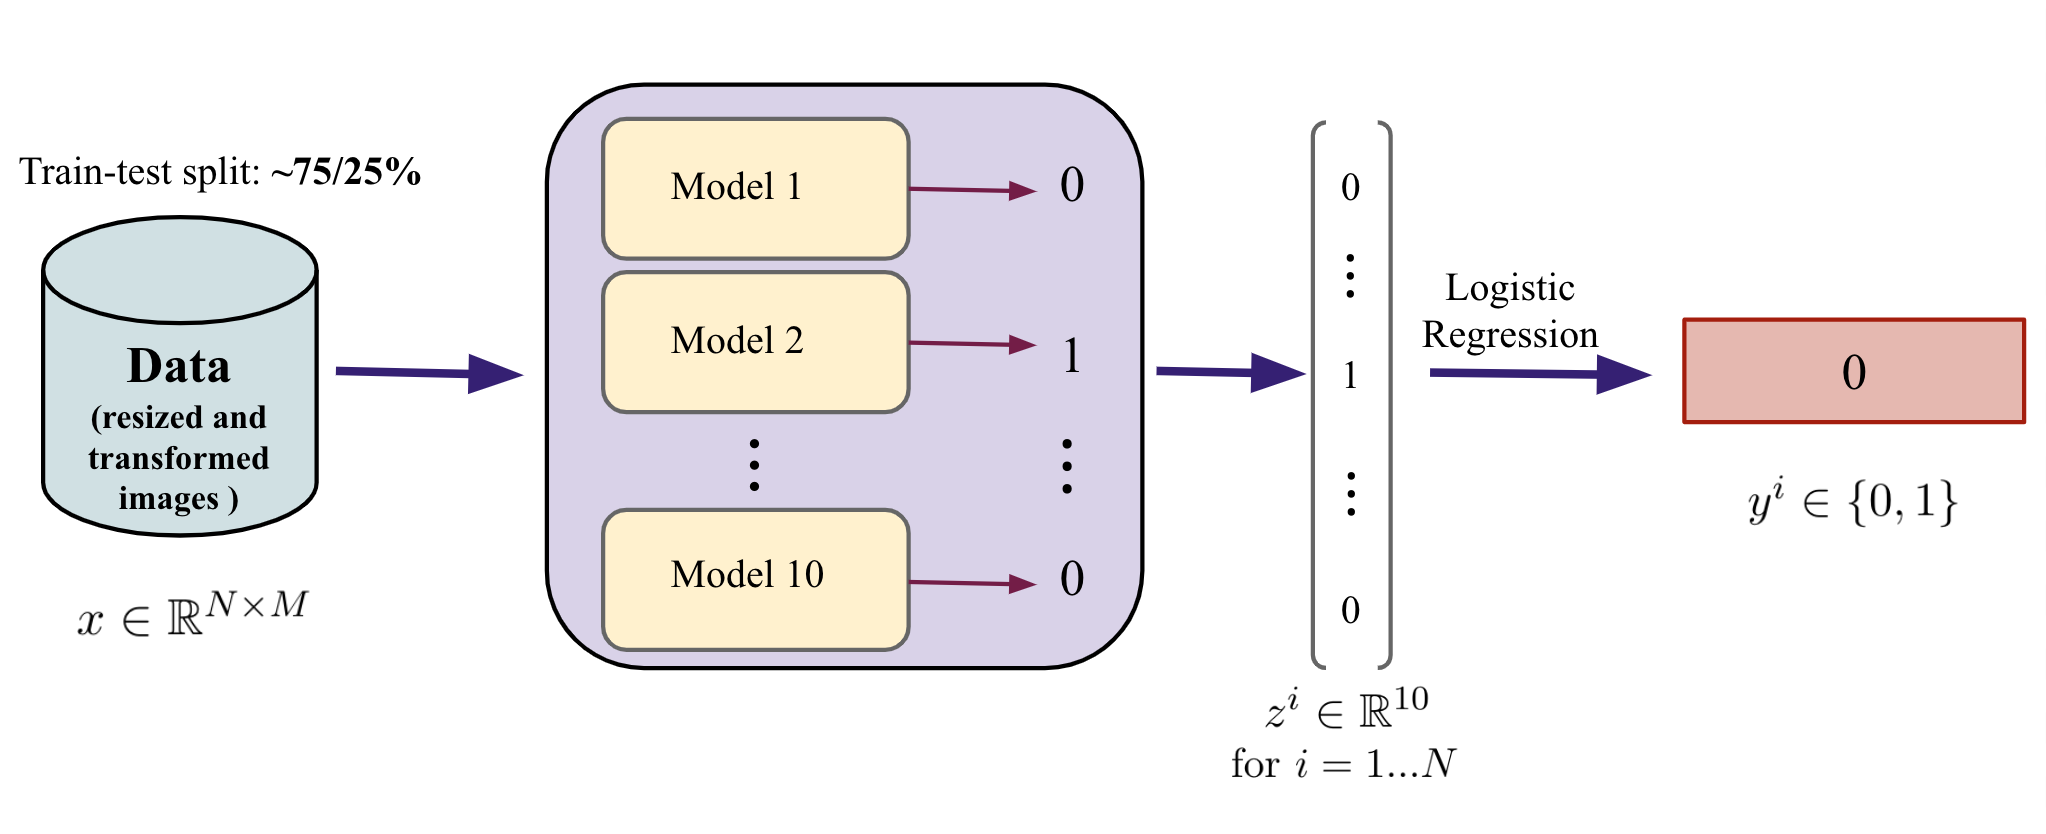
\includegraphics[scale=0.4]{images/stage2.png}
  \caption*{Training Stage 2.}
\caption[Ensemble Model]{The Architecture of the Ensemble Model. The input consists of $N$ observations with $M$ features. The ensemble produces a binary output of ``normal" or ``corrupted''. }
\label{fig:ensemble}
\end{figure}

\noindent 
Given the scope of this project, we were not able to apply all possible feature extraction and modeling combinations to all of the artifacts. Therefore, for each artifact, we thought about which feature representations can capture that artifact the best, and we only applied those methods. For example, there are no repetitive patterns in screen tearing artifacts so we did not consider using Fourier transform to extract features. Figure \ref{fig:methods-tried} illustrates what models we considered for each artifact.

\begin{figure}[!h]
  \centering
  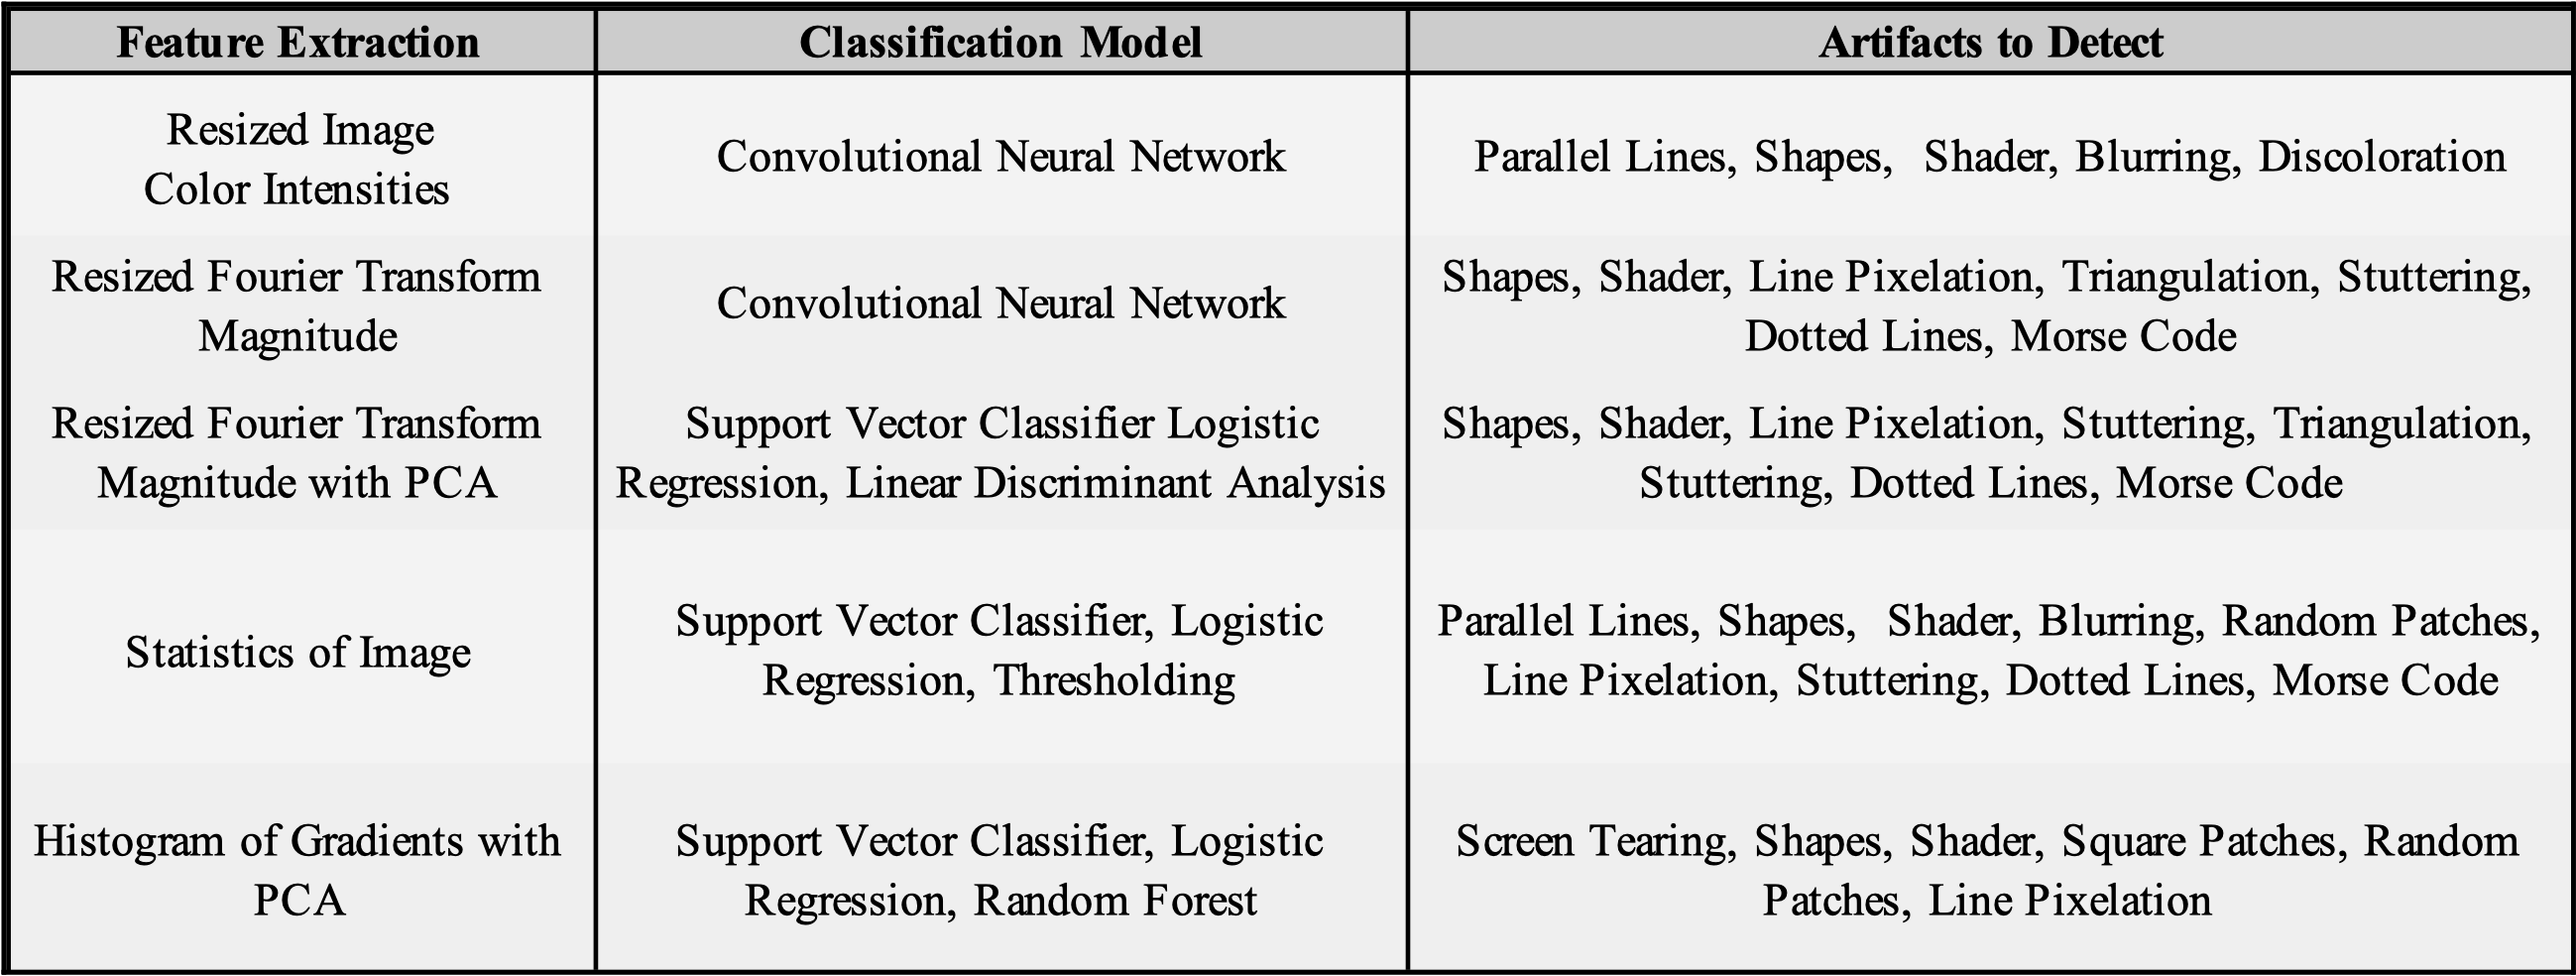
\includegraphics[scale=0.3]{images/results-methods.png}
  \caption{Methods we tried for each artifact.}
\label{fig:methods-tried}
\end{figure}


% \begin{comment}
% \begin{table}[!ht]
% \centering
% \begin{tabular}{@{}lllll@{}}
% \toprule
% Feature & Classification Model & Corruption Type  \\ \midrule
% Resized Image & 580 & 1070\\
% Resized FT (magnitudes) & 1241 & 409\\
% Resized FT (magnitudes) \& PCA & 832 & 818\\
% Image Statistics & 1641 & 9\\
% Histogram of Gradients & 1621 & 29\\\bottomrule
% \end{tabular}
% \caption[Individual model combinations]{Individual classifiers considered (selected combinations shown in bold).}
% \label{fig:methods-tried}
% \end{table}
% \end{comment}

\noindent 
We considered two input formats for the ensemble model---binary outputs of the individual classifiers and their raw probability vectors. In addition, we attempted to employ an $OR$ logic concatenation of the individual models, however, this yielded poor performance due to the cumulative effect of false positive rates of the individual models.\\

\noindent 
In addition to the ensemble structure explained earlier - in which the individual models have a binary output of 0 or 1 and a logistic regression is trained on those outputs - we considered a number of different approaches.
\begin{enumerate}
    \item\textit{Probabilities output of individual models}. n this case, instead of having each of the individual models output 1 or 0, we had them output a probability, and trained the logistic regression on those probability vectors (still in $\mathbb{R}^{10}$). If a model was not equipped with a probability output (i.e SVM) we just used the binary output.
    \item\textit{Using OR logic}. Instead of using a logistic regression to produce binary outputs for the ensemble model, we could also use the or logic. This means that for a given image, if at least one model flags it as ``corrupted", then the ensemble will flag that image as corrupted. In other words if the magnitude of $z^i$ in Figure \ref{fig:ensemble} is greater than 0, then the ensemble will flag the $i^{th}$ image as ``corrupted".
\end{enumerate}

\section{Performance Metrics}
In order to evaluate the performance of our models, we have adopted three different metrics: accuracy, precision and recall. Let an image that is predicted to contain glitches be ``positive" and an image that is predicted to be normal be ``negative." Then, if a glitched image is labeled as ``glitched" correctly, it is a true positive (TP); otherwise, it is a false negative (FN) if our model mislabels it as a normal image. Similarly, if a normal image is labeled as ``normal" correctly, it is a true negative (TN); otherwise, it is a false positive (FP) if our model mislabels it as glitched. The definitions of the three metrics are as follows:
\begin{align}
\text{Accuracy}&=\frac{\text{TP+TN}}{\text{TP+FP+TN+FN}},\\\nonumber
\text{Precision}&=\frac{\text{TP}}{\text{TP+FP}},\\\nonumber
\text{Recall}&=\frac{\text{TP}}{\text{TP+FN}}\nonumber.
\end{align}
\noindent In the next section, we will present the results of our classification models. The model performances are evaluated in terms of accuracy, precision and recall as defined above.

\endinput